\documentclass[crop,tikz]{standalone}
\usetikzlibrary{backgrounds}
\colorlet{blue}{cyan}
\tikzset{
  inverted/.style = {
    every path/.style = {draw=white,text=white},
    background rectangle/.style={fill},
    show background rectangle
  }
}

\tikzset{>=latex}
\usetikzlibrary{calc}
\colorlet{gray}{gray!60}

\begin{document}
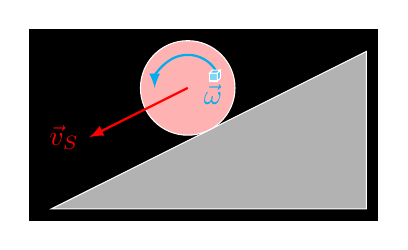
\begin{tikzpicture}[inverted,scale=2]
  \pgfmathsetmacro{\al}{atan(0.5)} % angle
  \pgfmathsetmacro{\sa}{sin(\al)}; % sin(angle)
  \pgfmathsetmacro{\ca}{cos(\al)}; % cos(angle)
  \pgfmathsetmacro{\radius}{0.3};  % radius
  % inclined plane
  \draw[fill=gray] (0,0) -- (2,0) -- (2,{2*tan(\al)}) -- cycle;
  % rotating body
  \coordinate (body) at ($(1,{tan(\al)})+(90+\al:\radius)$);
  \draw[fill=red!30] (body) circle (\radius);
  % arrows
  \draw[->,red,thick] (body) -- ++(180+\al:0.7) node[left] {$\vec{v}_S$};
  \coordinate (cube) at ($(body)+(\al:0.7*\radius)$);
  \draw[->,blue,thick] (cube) arc (\al:180:0.7*\radius);
  \node[below,blue] at ($(body)+(\al:0.6*\radius)$) {$\vec{\omega}$};
  % cube
  \pgfmathsetmacro{\cubex}{0.05}
  \pgfmathsetmacro{\cubey}{0.05}
  \pgfmathsetmacro{\cubez}{0.05}
  \draw[fill=blue!50] (cube) -- ++(-\cubex,0,0) -- ++(0,-\cubey,0) -- ++(\cubex,0,0) -- cycle;
  \draw[fill=blue!70] (cube) -- ++(0,0,-\cubez) -- ++(0,-\cubey,0) -- ++(0,0,\cubez) -- cycle
                      (cube) -- ++(-\cubex,0,0) -- ++(0,0,-\cubez) -- ++(\cubex,0,0) -- cycle;
\end{tikzpicture}%
\end{document}
